\chapter{Revisão Bibliográfica}

Neste capítulo é apresentada a revisão da bibliografia que dará suporte e embasamento para o desenvolvimento deste trabalho, expondo técnicas, conceitos fundamentais e tecnologias que são citadas na literatura para a resolução do problema proposto. Os principais fundamentos teóricos que são cruciais para a compreensão do trabalho são abordados na seção \ref{fundamentacao}. A proposta para o método de desenvolvimento do protótipo é discutida na seção \ref{metodo-desenvolvimento}. Por fim, alguns trabalhos relacionados são explorados na seção \ref{relacionados}, onde são destacadas as semelhanças, diferenças e contribuições para o trabalho.

\section{Fundamentação Teórica}\label{fundamentacao}
Nesta seção são apresentados conceitos fundamentais para a compreensão do presente trabalho. Inicialmente, é apresentada uma contextualização sobre o transporte de passageiros em veículos coletivos urbanos (\ref{transporte-urbano}). Posteriormente, problemas de otimização são introduzidos em \ref{problemas-de-otimizacao}, incluindo um problema clássico de otimização denominado \emph{Vehicle Routing Problem}, que é detalhado na subseção \ref{vrp}. 

As principais técnicas computacionais para a resolução de problemas de Otimização Combinatória, incluindo o Problema de Roteamento de Veículos são introduzidas na subseção \ref{tecnicas-computacionais} classificados em \ref{classes-np} e exploradas em \ref{gulosos} (Algoritmos Gulosos) \ref{metodos-exatos} (Métodos Exatos), \ref{heuristica} (Métodos Heurísticos) e \ref{metaheuristica} (Métodos Meta-Heurísticos). Por fim, sistemas de georreferenciamento citados na literatura são apresentados na subseção \ref{georreferenciamento}

\subsection{Transporte Coletivo Urbano}\label{transporte-urbano}
Existem diversos atributos na relação do passageiro com o transporte público coletivo, mas esses atributos são independentes e devem ser estudados de forma isolada. A resolução do Contran \cite{denatran} é feita para que o veículo fique de acordo com cada atributo, sendo eles:
\begin{itemize}
    \item confiabilidade;
    \item tempo;
    \item acessibilidade;
    \item conforto;
    \item segurança;
    \item custo (tarifas).
\end{itemize}

A tabela \ref{cotran-table} relaciona o atributo do serviço com a sua definição e um indicador equivalente para a sua avaliação.

\begin{table}[H]
\centering
\caption{Indicadores do serviço adequado. }
\resizebox{\textwidth}{!}{%
\begin{tabular}{ccccc}
\textbf{\begin{tabular}[c]{@{}c@{}}PARÂMETRO\\ DO SERVIÇO\\ ADEQUADO\end{tabular}} & \textbf{\begin{tabular}[c]{@{}c@{}}DEFINIÇÃO DO\\ PARÂMETRO\end{tabular}} & \textbf{\begin{tabular}[c]{@{}c@{}}INDICADOR\\ EQUIVALENTE\end{tabular}} & \textbf{SIGLA} & \textbf{\begin{tabular}[c]{@{}c@{}}DEFINIÇÃO\\ ADOTADA NO\\ INDICADOR\end{tabular}} \\ \hline
Regularidade & \begin{tabular}[c]{@{}c@{}}Prestação do serviço\\ conforme contrato, sem\\ interrupções\end{tabular} & Pontualidade & $P_N$ & \begin{tabular}[c]{@{}c@{}}Oferta do serviço de\\ forma contínua e\\ conforme planejado\end{tabular} \\ \hline
Continuidade & \begin{tabular}[c]{@{}c@{}}Manutenção da oferta\\ em caráter permanente\end{tabular} & Tempo & $T_E$ & \begin{tabular}[c]{@{}c@{}}Tempo de realização\\ da viagem, incluindo\\ transbordos\end{tabular} \\ \hline
Eficiência & \begin{tabular}[c]{@{}c@{}}Atendimento ao usuário\\ com o melhor uso dos\\ recursos\end{tabular} & Lotação & $L_O$ & \begin{tabular}[c]{@{}c@{}}Oferta de lugares e\\ conforto das viagens\end{tabular} \\ \hline
Segurança & \begin{tabular}[c]{@{}c@{}}Confiança oferecida ao\\ usuário na prestação do\\ serviço\end{tabular} & Segurança & $S_G$ & \begin{tabular}[c]{@{}c@{}}Serviço seguro, sem\\ incidência de\\ acidentes e assaltos\end{tabular} \\ \hline
Atualidade & \begin{tabular}[c]{@{}c@{}}Modernidade de\\ técnicas, equipamentos\\ e instalações\end{tabular} & Informações & $I_F$ & \begin{tabular}[c]{@{}c@{}}Uso de técnicas para\\ fornecer informação\\ ao usuário, sem\\ necessidade de\\ solicitação\end{tabular} \\ \hline
Generalidade & \begin{tabular}[c]{@{}c@{}}Serviço com\\ atendimento a todos os\\ usuários, sem distinções\end{tabular} & Veículos & $V_E$ & \begin{tabular}[c]{@{}c@{}}Acesso de pessoas\\ com necessidades\\ especiais e\\ conservação dos\\ veículos\end{tabular} \\ \hline
Cortesia & \begin{tabular}[c]{@{}c@{}}Serviço prestado com\\ urbanidade ao usuário\end{tabular} & Tripulação & $T_R$ & \begin{tabular}[c]{@{}c@{}}Comportamento dos\\ operadores e sua\\ relação com usuários\end{tabular} \\ \hline
\begin{tabular}[c]{@{}c@{}}Modicidade das\\ tarifas\end{tabular} & \begin{tabular}[c]{@{}c@{}}Tarifas compatíveis\\ com a renda do usuário\end{tabular} & Tarifa & $T_A$ & \begin{tabular}[c]{@{}c@{}}Representatividade\\ da tarifa na renda do\\ usuário\end{tabular} \\ \hline
\end{tabular}%
}
Fonte: \cite[p. 43]{MARTINS}
\label{cotran-table}
\end{table}

Apesar da forte relação com o passageiro, as composições homologadas são de viés automotivo e não pensados no lado do usuário.
 
Os atributos de tempo e capacidade dos veículos caracterizam o transporte urbano coletivo e estão ligados no projeto do veículo, que são prefixados pelos fabricantes. Para o passageiro,o aspecto conforto é composto por um veículo com pouca ocupação, garantindo que o passageiro estará sentado durante a viagem, mas o que também faz parte da satisfação do usuário é a extensão do deslocamento.

A figura a seguir representa a relação entre a densidade de ocupação de um veículo (em pessoas por $m^2$) e o tempo de deslocamento (em minutos).

\begin{figure}[H]
  \centering
  \caption{Relação entre densidade de ocupação e tempo de deslocamento}
 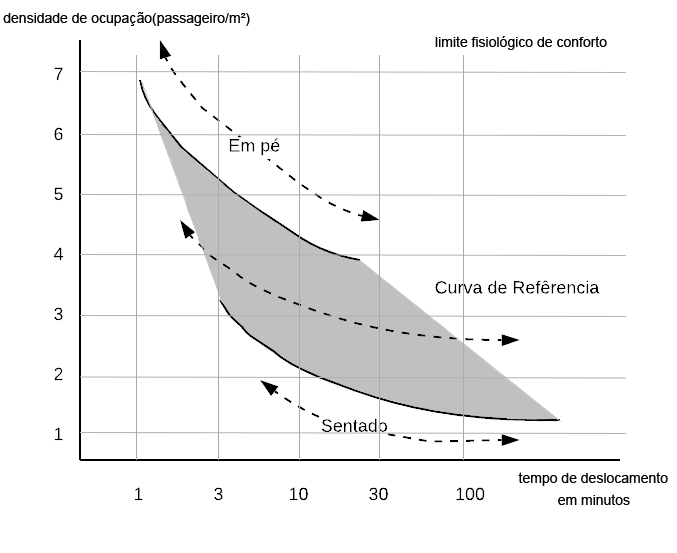
\includegraphics[scale=0.55]{imagens/limite-fisiologico.png} \par
\bigskip
Fonte: \cite[p.307]{MARTINS}
\end{figure}
Assim, em relação ao transporte de passageiros, os princípios que devem estar presentes para um bom nível de serviço, em destaque, são: 
\begin{itemize}
    \item \textbf{Permanência}: um serviço constante, sem problemas de prestação de serviços.
    \item \textbf{Eficiência}: oferta de um serviço satisfatório (conforto).
    \item \textbf{Modicidade}: serviços a preços razoáveis
\end{itemize}

\subsection{Problemas de Otimização}\label{problemas-de-otimizacao}

Problemas de otimização podem ser fundamentalmente divididos entre aqueles com variáveis contínuas ou de natureza discreta \cite{combinatorial-optimization}. Nos problemas de otimização de variáveis contínuas procura-se por uma função ou um conjunto de números \(R \in \textrm I\!R \) para a solução.

Já os problemas de otimização de natureza discreta podem ser solucionados por meio de técnicas de Otimização Combinatória. Nos Problemas de Otimização Combinatória procura-se um conjunto finito de soluções -- naturalmente inteiras -- e que podem ser formulados como Problemas de Programação Inteira e consequentemente solucionados por meio de Algoritmos de Programação Inteira \cite{goldbarg} ou podem ser formulados por meio de análise combinatória e solucionados como problemas em Grafos ou algoritmos especificamente desenvolvidos.


Problemas de Otimização Combinatória podem ser formulados como \((F, c)\) onde \(F\) é um conjunto de pontos possíveis; e \(c\) uma função de custo \cite{rodolfo}.

\[c: F \longrightarrow R^1 \]

Onde o problema é encontrar um\(f \in F\) para qual

\[c(f) \leq c(y): y \in F \]

O ponto \(f\) é denominado de ótimo global ou solução ótima.

\subsubsection{Vehicle Routing Problem (VRP)} \label{vrp}

O Problema de Roteamento de Veículos (Vehicle Routing Problem - VRP) é um problema clássico de otimização combinatória que foi introduzido na literatura em 1959 por Dantzig e Ramser \cite{toth}. O VRP tem sido, particularmente, um dos problemas mais abordados nas áreas de Otimização Combinatória e Pesquisa Operacional nas últimas décadas (artigo sobre transporte escolar). E desde então, vários cenários foram derivados, como o roteamento para veículos de entrega, roteamento de veículos escolares ou o roteamento de veículos para transporte de passageiros no contexto urbano, que é o objeto de estudo do trabalho presente. De modo geral, consiste em definir rotas para cumprimento de demandas, considerando o número de veículos disponíveis e respeitando a capacidade de cada veículo.

O problema de roteamento de veículos abertos (\emph{Open Veihicle Routing Problem} -- \emph{OVRP}) é um existentes na derivação do \emph{VRP}. O \emph{OVRP} consiste em caminhos hamiltonianos para um conjunto de clientes atribuídos num mesmo veículo a partir de uma demanda total de todos os clientes de uma rota e que não deve exceder capacidade do veículo; cada cliente é visitado apenas uma vez por um dos veículos. Porém, o \emph{OVRP} é dado como problema de coleta e entrega de carga e não propriamente de passageiros.

No problema em questão, a partir de passageiros coincidentes de uma região, o objetivo é transportá-los para um local próximo ao seu destino, minimizando custos e melhorando frotas para atendimento de regiões condizentes. 

Tendo em vista ser uma problema de otimização e combinatória, há diversas maneiras de solução, seja com algoritmos gulosos ou por soluções exatas, heurísticas e metaheurísticas. Antes mesmo de entender os tipos de soluções, existe as classes que os algoritmos podem pertencer e, assim, é possível decidir qual deles é mais adequada de acordo com a solução para o seu problema.

\subsection{Técnicas Computacionais para Resolução de Problemas de Otimização Combinatória}
\label{tecnicas-computacionais}
O desenvolvimento da capacidade de processamento dos computadores nos últimos anos tem servido de suporte para a solução -- mesmo que parcial -- de problemas de Otimização Combinatória, algumas vezes envolvendo centena de milhares de variáveis e restrições.

Diferentes métodos podem ser utilizados para a solução do VRP, que fundamentalmente a literatura os separa entre três principais classes: Métodos Exatos, Métodos Heurísticos e Meta-Heurísticos \cite{maxwell}. Antes mesmo de abordar os tipos de soluções, é necessário entender as classes que os algoritmos podem pertencer e, assim, será possível escolher os melhores candidatos para a solução do problema proposto. Nas subseções seguintes, um levantamento dos métodos mais frequentes para a solução foi realizado a fim de guiar na decisão da escolha da abordagem para resolver o problema proposto pelo trabalho.

\subsection{NP-Completo e NP-Difícil}
\label{classes-np}

A classe NP (\emph{nondeterministic polynomial time}) é a classe de linguagens decidíveis que podem ser verificadas por um algoritmo em tempo polinomial. O problema do Caixeiro Viajante, por exemplo, tem complexidade $O(n!)$, porém essa complexidade pode ser diminuída até $O(n^22^n)$ com programação dinâmica. A definição de acordo com Nivio Ziviani (\citeyear{ziviani}):

\begin{quote}
Apenas problemas de decisão (“sim/não”) podem ser \emph{NP-Completo}.
\end{quote}
\rightline{\cite[p. 415]{ziviani}}

Assim, se uma classe \emph{NP-completo} pode ser resolvido em tempo polinomial a partir de uma máquina determinística, então todos os problemas da classe podem. Isto é, a classe \emph{P} é igual a classe \emph{NP}. Essa afirmação ainda não foi comprovada com nenhum problema da classe \emph{NP-Completo}.

Um problema A pertence a classe \emph{NP-Difícil} se existe um problema $B \in $ \emph{NP-Completo} que pode ser transformado em A em tempo polinomial. Portanto, a única diferença com relação à classe \emph{NP-Completo} é que A não é provado ser \emph{NP}.
\cite[p. 4]{bueno}

Concluindo que o problema que pertence à classe \emph{NP-difícil} não é provado ser resolvido em tempo polinomial.

\subsection{Algoritmos Gulosos}
\label{gulosos}
Algoritmos com estratégia gulosa (=gananciosa =\emph{greedy}) \cite{feofiloff} são os relacionados com problemas de otimização que não repensam a solução tomada, assim, tomando-as com base na informação disponível sem se preocupar com efeitos futuros. 

\begin{quote}
Não existe necessidade de avaliar alternativas, nem de empregar algoritmos sofisticados que permitam desfazer decisões tomadas previamente. A razão de o algoritmo ser chamado guloso é que o algoritmo escolhe, a cada passo, o candidato mais evidente que possa ser adicionado à solução.
\end{quote}
\rightline{\cite[p. 58]{ziviani}}

\subsection{Métodos Exatos} \label{metodos-exatos}

Em métodos exatos uma varredura é realizada sobre todo o domínio de busca das soluções, garantindo que o ótimo global seja encontrado sempre que a solução for viável. Entretanto, algoritmos de métodos exatos não podem ser executados em tempo polinomial, de forma que a equação de tempo em função dos número de insumos cresce de forma polinomial \cite{maxwell}. São explorados a seguir alguns métodos exatos mais citados pela literatura para resolver o VRP.

\subsubsection{Branch-and-bound}
Esta estratégia consiste em solucionar problemas de otimização com restrições de variáveis inteiras. A partir de um problema inicial, é criada uma série de ramificações (\emph{Branch}) das restrições (\emph{Bound}) que existem neste problema, de modo que, as restrições não permitam uma solução parcial do problema. Esta estratégia monta uma árvore de decisão com base em limites superiores e inferiores, impedindo que algumas soluções ruins sejam exploradas. Este método pode ser utilizado com outros métodos de programação linear, como por exemplo, o SIMPLEX \cite{LAPORTE1992345}. O \emph{Branch-and-Bound} elimina ramificações de restrições caso se encontre uma das condições:

\begin{enumerate}
    \item O problema restrito é impossível.
    \item A solução ótima do ramo é inteira.
    \item A solução encontrada no ramo é pior do que a melhor solução atual.
\end{enumerate}

\subsubsection{Branch-and-cut}
Esta estratégia é uma melhoria do algoritmo \emph{Branch-and-bound}. Nela, ocorre a resolução dos problemas relaxados (sem restrições de integralidade) do \emph{Branch-and-bound}, utilizando um plano de cortes. O algoritmo passa nó a nó da árvore, executando o plano de cortes e checando se naquele nó, a solução ótima do subproblema obedece às restrições de integralidade ou se o limitante inferior é maior que a solução já conhecida, caso uma dessas situações ocorra, o nó é descartado. Caso não seja encontrada uma inequação válida para o problema de separação, aplica-se a ramificação.


\subsubsection{Branch-and-price}
Em casos de problemas de otimização com variáveis integrais, onde se considera todas as variáveis do problema simultaneamente, torna-se inviável a utilização das estratégias anteriores. Visto esse tipo de problema, foi criada uma técnica chamada de Geração de Colunas, com intuito de resolver esse tipo de problema. A técnica visa selecionar variáveis com o maior potencial para otimizar o problema. A estratégia \emph{Branch-and-price} é uma versão da estratégia \emph{Branch-and-bound}, que utiliza a Geração de Colunas  em cada nó da árvore de decisão.

\subsection{Métodos heurísticos}\label{heuristica}
A etimologia da palavra \emph{heurística} tem origem do verbo grego \emph{heuriskein} -- cuja conjugação na primeira pessoa é \emph{eureka} -- que significa descobrir. No entanto, quando a palavra é empregada no contexto de métodos para a solução de problemas de Otimização Combinatória, o seu sentido pode ser ampliado conforme, por exemplo, a definição de Kendra van Wagner-Cherry \emph{``Uma heurística é um atalho mental que permite às pessoas resolver problemas e fazer julgamentos rápida e eficientemente.''} \cite{goldbarg}


Métodos heurísticos são aqueles as que garantem um bom tempo computacional, porém, não garantem uma solução ótima em todos os casos que atuam. No caso de uma aplicação, uma aproximação heurística traz o benefício do tempo de processamento, uma vez que uma solução ótima, com alto tempo de processamento, deixa de ser uma boa solução para o usuário. 

A seguir, alguns exemplos de estratégias heurísticas para o VRP.

\subsubsection{Clarke e Wright}

Esta foi uma estratégia extremamente importante para o desenvolvimento dos algoritmos voltados ao VRP, este algoritmo serviu como base para a construção de outros algoritmos sofisticados de roteamento de rotas e veículos \cite{milton-nascimento}. O algoritmo cria grafos contendo os clientes e possíveis rotas, já o depósito é lido a partir de alguma estrutura de armazenamento, então, são calculadas \emph{n-1} rotas de um cliente ao depósito onde n é o número de nós do grafo. A partir destes pares de nós, é calculado  o custo da rota a partir da fórmula \cite[p. 32]{maxwell}: 

\[ s_{ij} = c_{i0} + c_{0j} - c_{ij} \]

Onde $s_{ij}$ representa a economia com relação aos nós \emph{i} e \emph{j}, e $c_{ij}$ representa o custo de se ir do nó \emph{i} ao nó \emph{j}. As economias são colocadas, em ordem decrescente, em uma tabela após o cálculo. 

O algoritmo de \emph{Clark e Wright} é resolvido em tempo polinomial, pois, a complexidade é da ordem $\mathcal{O}(n^2)$. Há, no entanto, uma desvantagem de se usar a estratégia de \emph{Clark e Wright}, pois o algoritmo descartará todos os nós que não se encontram nos extremos das rotas, ou seja, os nós internos não entram na tabela de economia.

\subsubsection{Mole e Jameson}

A estratégia de \emph{Mole e Jameson} é uma melhoria do algoritmo de \emph{Clark e Wright}, ele tem como um ponto forte, considerar os nós internos que são descartados no teste de economia do algoritmo de \emph{Clark e Wright}. O algoritmo começa carregando o grafo a partir de uma matriz de adjacências e de uma lista de nós livres (nós que não pertencem à nenhuma rota). Posteriormente, é construído um grafo que não contém o nó do depósito a partir da matriz de adjacências e da lista de nós livres. A partir de algum critério pré-definido, um par de nós é escolhido para ser a rota inicial. Após definida a rota inicial, um laço começará a inserir os nós na rota, seguindo dois critérios: O de \textbf{Proximidade} e o de \textbf{Economia}.
Para realizar o cálculo da \textbf{Proximidade} dos nós é utilizada a seguinte fórmula \cite[p. 33]{maxwell}:

\[\alpha(i, k, j) = c_{ik} + c_{kj} - \lambda c_{ij} \]

Onde $c_{ik}$ representa o custo entre os nós \emph{i} e \emph{k}, $c_{kj}$  representa o custo entre os nós \emph{l} e \emph{j}. Se nenhuma violação for quebrada, o nó com menor distância será inserido na rota. O cálculo da economia é aquele que apontará qual o melhor lugar para o nó ser inserido, este cálculo é dado por:

\[\beta(i, k, j) = \mu 0k - \alpha(i, k, j) \]


Onde \(\mu 0k\) representa a distância entre o depósito e o nó $l$. O local selecionado representa o que tem mais economia.

\subsection{Métodos meta-heurísticos}\label{metaheuristica}
O prefixo \emph{meta} é de origem grega e seu significado original é \emph{além}. Entretanto, em diversas áreas de conhecimento, o seu uso normalmente é empregado para fornecer um significado sobre algo de sua própria natureza, como um conceito que é uma abstração que explica um outro conceito. Desta forma, \emph{meta-heurísticas} são heurísticas projetadas para encontrar, gerar, ou selecionar heurísticas.

Formalmente, uma meta-heurística é composta por um conjunto de regras estruturadas que podem servir de base para a projeção da solução a partir de uma gama de heurísticas computacionais. Estratégias genéricas derivadas de heurísticas  podem ser aplicadas em variados contextos de problemas de otimização a partir de adaptações para resolver um problema específico \cite{maxwell}. Muitas meta-heurísticas são inspiradas em fenômenos naturais, como a Colônia de Formigas ou Enxame de Abelhas. Assim como na heurística, a solução ótima não é garantida nos métodos meta-heurísticos. A definição de Goldbarg \emph{et al.} (2015) indica o agrupamento de heurísticas computacionais para compor um sistema geral de regras: 

\begin{quote}
Trata-se de uma arquitetura geral de regras que, formada a partir de um tema em comum, pode servir de base para o projeto de uma ampla gama de heurísticas computacionais.
\end{quote}
\rightline{\cite[p. 75]{goldbarg}}

A figura \ref{heuristica-goldbarg} exibe características genéricas de uma abordagem meta-heurística (indicado na figura como Regras Gerais) para agrupar e adaptar heurísticas de determinado tema em comum para a resolução de mais de um problema dentro do contexto dos Problemas de Aplicação.

\begin{figure}[H]
  \centering
  \caption{Arquitetura geral para meta-heurísticas}
 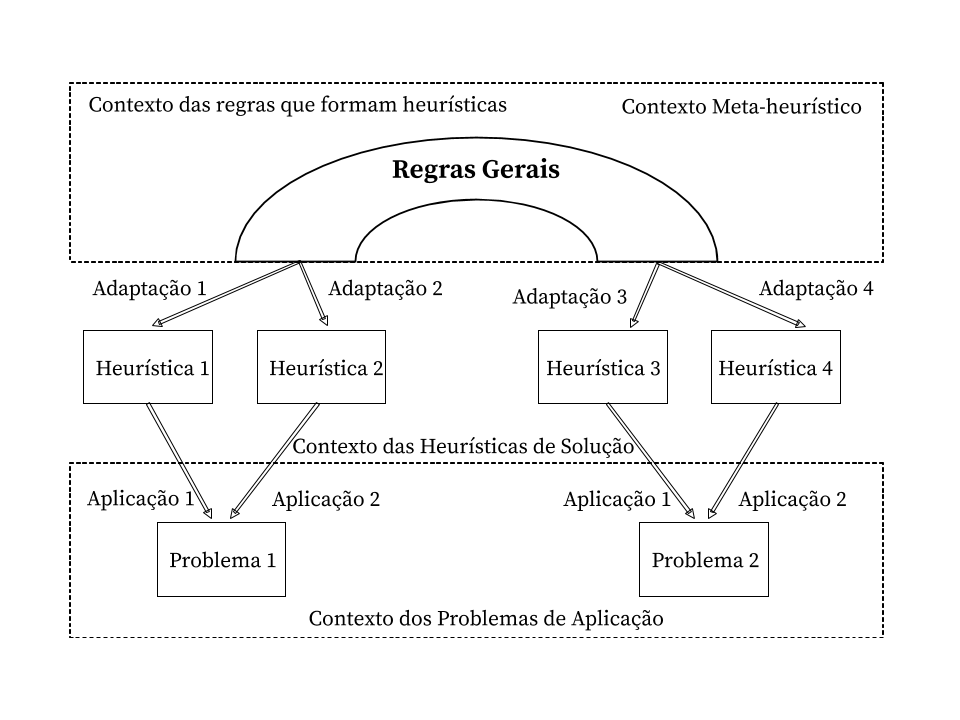
\includegraphics[scale=0.4]{imagens/metaheuristica.png} \par
\bigskip
\label{heuristica-goldbarg}
    \cite[p. 75]{goldbarg}
\end{figure}

A seguir, são apresentadas algumas abordagens meta-heurísticas que a literatura já utilizou dentro do contexto do VRP.

\subsubsection{Busca Tabu}

A etimologia da palavra \emph{tabu} tem origem do \emph{Tongan}, idioma falado em Tonga, na Polinésia e indica algo proibido por ser sagrado e que não pode ser tocado ou mencionado. O algoritmo da busca tabu é assim nomeado por ser composto de estratégias que permitem \emph{proibir} determinadas ações durante a varredura de vizinhanças e a escolha de soluções.

A busca tabu foi introduzida na literatura por Fred Glover em 1986 \cite{GLOVER1986533} e posteriormente aperfeiçoada em outros trabalhos acadêmicos. É um método que permite tanto uma abordagem probabilística \cite{crainic1993dynamic} quanto determinística \cite{ongsakul2004unit}. Ao contrário de muitos métodos meta-heurísticos, a busca tabu não possui analogia com um fenômenos naturais. Os princípios de uma busca tabu segundo Golbarg \emph{et al.} (2015) são:
\begin{enumerate}
    \item Uma busca eficiente não deve revisitar soluções;
    \item Manter registro de todas as soluções visitadas é computacionalmente dispendioso. É mais eficiente armazenar alterações na solução ou em variáveis; e
    \item Memorizar alterações nas soluções não elimina a possibilidade de reexame de soluções, apenas diminui a chance dessa possibilidade.
\end{enumerate}

Um dos princípios da busca tabu é aproveitar-se de um esquema de gestão de memória auxiliar de curto, médio e longo prazo para evitar examinar mais de uma vez uma mesma configuração em uma varredura em busca de uma solução. Este conjunto de proibições -- usualmente denominado \emph{condições tabu} -- é registrado em memória dinâmica, permitindo que seja alterado de acordo com o progresso da busca, visto que podem ocorrer evidências de que uma configuração de solução não está sendo considerada e estas proibições precisam ser desativadas. Além de evitar repetições, uma otimização das configurações da busca permite aumentar a chance da busca escapar da atração de mínimos locais. 

Fundamentalmente, algoritmos de busca tabu são orientados à varredura de vizinhanças específicas (denominada \emph{intensificação}) com configuração de foco de busca variável (denominada \emph{diversificação}). Um algoritmo de busca tabu visa crucialmente minimizar a quantidade de configurações visitadas e fornecer condições de escape de mínimos locais. Portanto, para atingir este objetivo, uma busca tabu é composta por:

\begin{itemize}
    \item Memória de curto prazo para preservar o histórico imediato da busca;
    \item Estratégias de memória de médio e longo prazo com o objetivo de equilibrar o esforço computacional da \emph{intensificação} com o utilizado na \emph{diversificação};
    \item Regras que permitam ajustar gestão da memória, critérios de pertubação e de escolha da configuração.
\end{itemize}

A busca tabu armazena na memória algumas soluções e armazena as alterações posteriores nas próprias soluções. Estas modificações nas soluções são denominadas de \emph{pertubações}. Uma \emph{pertubação} é uma alteração no valor ou na composição das variáveis de uma solução. Goldbarg \emph{et al.} (2015) exemplificam alguns exemplos de possíveis movimentos em uma configuração:

\begin{itemize}
    \item Mudar as atribuições de uma variável binária de zero para um, ou vice-versa.
    \item Permutar os vértices em uma solução de rota.
    \item Introduzir ou retirar arcos em uma grafo solução.
    \item Alterar as atribuições realizadas sobre os vértices de um grafo solução.
\end{itemize}

A figura \ref{taboo-image} representa através de um fluxograma o passo a passo de um algoritmo de Busca Tabu. Os comentários identificam o propósito e o nome de cada passo. 


\begin{figure}[H]
  \centering
  \caption{Passo a passo com comentários de um algoritmo de Busca Tabu.}
 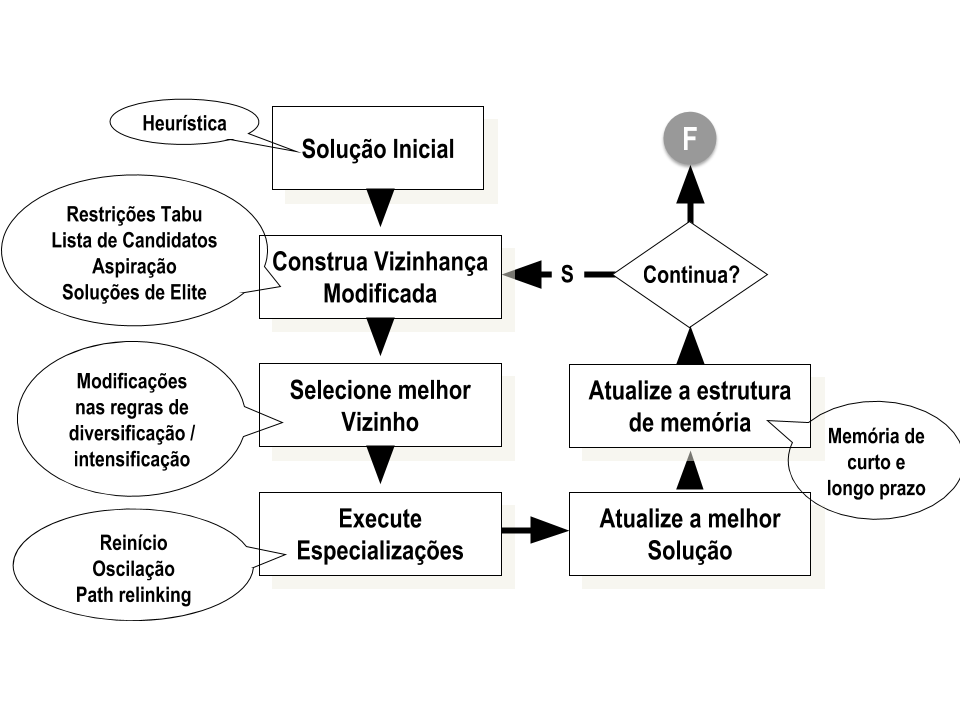
\includegraphics[scale=0.4]{imagens/tabu.png} \par
\bigskip
    \cite[p. 97]{goldbarg}
    \label{taboo-image}
\end{figure}


\textbf{Pseudocódigo da Busca Tabu} \par

O Algoritmo 1 representa em pseudocódigo, um algoritmo de busca tabu. A variável $p_{max}$ controla o máximo de iterações. A variável $q_{max}$ controla as iterações sem melhoria. \emph{N(s)} simboliza a vizinhança da configuração \emph{s} e \emph{f(s)} representa o valor da configuração \emph{s}.

\makeatletter
\renewcommand{\ALG@name}{Algoritmo}
\makeatother
\renewcommand{\listalgorithmname}{Lista de Algoritmos}

\algrenewcommand\algorithmicend{\textbf{fim}}
\algrenewcommand\algorithmicdo{\textbf{faça}}
\algrenewcommand\algorithmicwhile{\textbf{enquanto}}
\algrenewcommand\algorithmicfor{\textbf{para}}
\algrenewcommand\algorithmicif{\textbf{se}}
\algrenewcommand\algorithmicthen{\textbf{então}}
\algrenewcommand\algorithmicelse{\textbf{senão}}
\algrenewcommand\algorithmicreturn{\textbf{devolve}}
\algrenewcommand\algorithmicfunction{\textbf{função}}
\algrenewtext{EndWhile}{\algorithmicend\ \algorithmicwhile}
\algrenewtext{EndFor}{\algorithmicend\ \algorithmicfor}
\algrenewtext{EndIf}{\algorithmicend\ \algorithmicif}
\algrenewtext{EndFunction}{\algorithmicend\ \algorithmicfunction}
\algnewcommand\algorithmicto{\textbf{até}}
\algrenewtext{For}[3]%
{\algorithmicfor\ #1 $\gets$ #2 \algorithmicto\ #3 \algorithmicdo}
\begin{algorithm}
\caption{Busca tabu \cite[p. 89]{goldbarg}} 
\begin{algorithmic}[1]
\item \textbf{gerar} uma solução inicial \emph{s}, e fazer \emph{s}* := \emph{s}
\item \textbf{inicializar} a Lista Tabu (T)
\item \textbf{inicializar} contadores \emph{p} e \em{q}

\While{$p \neq p_{max}$ e $q \neq q_{max} $}
    \State \textbf{selecionar} o melhor vizinho $s' \in N(s) \setminus T$ 
    \State \textbf{selecionar} o melhor vizinho $s'' \in N(s) \cap T$ 
    \State \If{$f(s'') < f(s') $ e $f(s'') < f(s^*)$}
    \State {$s' \gets s''$}  \Comment{Aspiração} 
    \EndIf
    
    \State \If{$f(s') < f(s^*)$}
    \State {$s^* \gets s'$}
    \State {$q \gets 0$}
    \EndIf
    
    \State \If{$f(s') < f(s)$}
    \State \textbf{colocar} o movimento inverso $(s', s)$ na lista \emph{T}
    \State \textbf{atualizar} \emph{T}
    \EndIf
    
    \State{$s \gets s'$}
    \State{$p \gets p+1$}
    \State{$q \gets q+1$}
\EndWhile
\item \textbf{Devolver} a solução \emph{s}*
\label{pseudocodigo-busca-tabu}
\end{algorithmic}
\end{algorithm}

\textbf{Busca Tabu na Literatura} \par
Na tabela \ref{tabu-relacionados} são listadas algumas referências de trabalhos acadêmicos relacionados que já utilizaram métodos da busca tabu encontrar a solução.

\begin{table}[ht]
\centering
\caption{Utilização de meta-heurística para a resolução do VRP}
\resizebox{\textwidth}{!}{%
\begin{tabular}{ccc}
\hline
\textbf{Referência} & \textbf{Tema} \\ \hline

\cite{TAILLARD1991443} & \begin{tabular}[c]{@{}c@{}}Robust taboo search for the quadratic\\ assignment problem\end{tabular} \\ \hline

\cite{TSUBAKITANI1998113} & An empirical study of a new metaheuristic for the traveling salesman problem \\ \hline

\cite{eglese} & Open vehicle routing problem \\ \hline

\cite{Marinakis2010} & Honey Bees Mating Optimization algorithm for large scale vehicle routing problems \\ \hline

\cite{MARINAKIS20114684} & Honey bees mating optimization algorithm for the Euclidean traveling salesman problem \\ \hline

\cite{DIAS2014122} & An Inverted Ant Colony Optimization approach to traffic \\ \hline

\cite{ESCARIO2015390} & Ant Colony Extended: Experiments on the Travelling Salesman Problem \\ \hline
\end{tabular}%
}
Fonte: Elaborado pelos autores.
\label{tabu-relacionados}
\end{table}

\subsubsection{Colônia de Formigas e Enxame de Abelhas}
Conforme dito anteriormente, muitos métodos meta-heurísticos são inspirados em fenômenos químicos, biológicos, sociais e naturais, como é o caso da Colônia de Formigas e Enxame de Abelhas. Algoritmos em Colônia de Formigas e Enxame de Abelhas são pautados na capacidade de como organismos simples com conceitos modestos de inteligência -- geralmente associados a insetos ou animais de cognição simples -- são capazes de atuar socialmente em conjunto e criar uma organização robusta.

Esta forma de organização social com razoável grau de autonomia é denominado de \emph{Inteligência Coletiva} e um dos precursores do estudo foi William Morton Wheeler, em 1911. Esta forma de inteligência é tão extraordinária que o Prêmio Nobel de 1911, Maurice Maeterlinck, já questionava em seu livro \emph{La Vie des Abeilles} e vários estudos posteriores foram realizados com os mais diversos tipos de insetos \cite{Dorigo2010}. A definição segundo Bonabeau \emph{et al.} \cite{bonabeau1999swarm}:

\begin{quote}
Inteligência Coletiva é uma abordagem que permite o desenvolvimento de algoritmos de processamento distribuído inspirados no comportamento de insetos sociais ou de outras sociedades animais.
\end{quote}
\rightline{\cite[p. 7]{bonabeau1999swarm}}

Na área de Otimização Combinatória, os precursores na utilização da Colônia de Formigas foram Beckers \emph{et al.} \cite{Beckers1992TrailsAU}, onde foi demonstrado através de um experimento que formigas são capazes de encontrar o caminho mais curto entre o formigueiro e uma fonte de alimentação explorando coletivamente o feromônio que as formigas deixam no chão enquanto caminhavam; e Colorni \emph{et al.} \cite{colorni1992distributed}, que ainda em 1992 publicaram estudo sobre otimização distribuída baseado em Colônias de Formigas.

Sob o ponto de vista sistêmico, estes algoritmos trabalham através de processos de auto-organização. A auto-organização pode ser atribuída a um sistema aberto -- um sistema que permite troca de energia com o ambiente -- que contém a propriedade de conseguir crescer em complexidade de forma organizada sem que exista um guiamento centralizado ou gestão externa ao sistema.

Os sistemas auto-organizados emergem padrões. Um padrão é um arranjo privado e organizado de objetos que é preservado no espaço e no tempo. Quando emergentes, estes arranjos permitem que as propriedades do sistema se alterem de forma organizada.

O processo que se opõe à desorganização (\emph{entropia}) é denominado de \emph{negentropia} ou \emph{sintropia}. O Nobel da Física Erwin Schrödinger, distinguiu sistemas com tendências entrópicas e outros que possuem dispositivos negentrópicos e que são capazes de se organizar em níveis cada vez mais complexos e se auto-organizar e regenerar. 

Os algoritmos de Colônia de Formigas são compostos de agentes (\emph{formigas}) que cooperam globalmente para encontrar uma solução. À medida que as soluções são construídas, estruturas de vizinhança ou especiais são marcadas como forma de comunicação. Essa comunicação é empregada assim como a utilização de feromônios na organização das formigas para a construção de uma solução aos passos da formiga que está procurando alimento. Desta forma, a construção da solução percorre uma trilha de decisões marcadas anteriormente.

Algoritmos de Colônia de Formigas seguem algumas características importantes:
\begin{itemize}
    \item As formigas não se comunicam diretamente;
    \item Cada formiga constrói uma solução movendo-se em uma sequência finita de estados.
    \item Estes movimentos são feitos de acordo com probabilidade que leva em consideração informações da própria formiga (memória simples de ações locais) e da trilha de feromônio (ações globais)
\end{itemize}

\begin{table}[H]
\centering
\resizebox{\textwidth}{!}{%
\begin{tabular}{cc}
\hline
\textbf{Referência} & \textbf{Tema} \\ \hline
\cite{DIAS2014122} & An Inverted Ant Colony Optimization approach to traffic \\ \hline
\cite{ESCARIO2015390} & Ant Colony Extended: Experiments on the Travelling Salesman Problem \\ \hline
\cite{Marinakis2010} & Honey Bees Mating Optimization algorithm for large scale vehicle routing problems \\ \hline
\cite{MARINAKIS20114684} & Honey bees mating optimization algorithm for the Euclidean traveling salesman problem \\ \hline
\end{tabular}%
}
\caption{Trabalhos relacionados que utilizaram práticas de colônia de formigas.}
\label{colonia-relacionados}
\end{table}

\subsubsection{Busca em uma Vizinhança Grande Adaptada}

\subsection{Sistemas de Georreferenciamento}\label{georreferenciamento}
A empresa Google fornece uma vasta gama de ferramentas de geolocalização que contribuem para o desenvolvimento de vários aplicativos e softwares que tem como objetivo guiar o usuário de alguma forma à um destino. Dentre elas, temos algumas APIs que se destacam quando se tem como objetivo, criar uma plataforma de roteamento veicular, sendo elas:
\begin{itemize}
    \item Google Places API - É um serviço que retorna informações sobre um lugar a partir de requisições HTTP, Lugares são definidos nessa API como estabelecimentos, localizações geográficas ou pontos de interesse proeminentes.
    
    \item Google Directions API - Fornece rotas de transporte público, bicicleta, carro e a pé. Calcula os tempos de deslocamento atuais ou futuros com base no trânsito em tempo real.
    
    \item Google Distance Matrix API - Fornece tempos de deslocamento e distâncias para um ou mais locais.
    
    \item Google Geocoding API - Transforma dados de endereço de ruas em dados de altitude e latitude
    
    \item Google Maps Embed API - Realiza a inclusão de uma interface gráfica de mapeamento da própria Google.

\end{itemize}

Esses serviços terão um papel importante no desenvolvimento da plataforma de roteamento de transportes coletivos, o uso dessas ferramentas facilita a entrada de informações na plataforma, e gera mais consistência na montagem da parte programática do projeto em questão.

\section{Método de Desenvolvimento}
\label{metodo-desenvolvimento}
Nesta seção, é detalhado o método de desenvolvimento para a implementação da solução e do protótipo seguindo conceitos de engenharia de software e modelagem.

\subsection{Iconix}
O ICONIX é um método de desenvolver software dentre os métodos ágeis composta pelas atividades Análise de Requisitos, Análise Preliminar, Projeto e Implementação. É um método simplificado que divide todas as fases de modelagem em duas visões iterativas: dinâmica e estática. 

A primeira atividade, Análise de Requisitos, é a fase que se envolve o início do projeto. A primeira tarefa é a conversa com o cliente, público alvo do projeto e todos interessados do projeto. Essa conversa resultará em inúmeros requisitos que darão uma estimativa de como deve ser a estruturação do projeto, visto que nesta fase, o projeto ainda não está estruturado.
O passo seguinte da análise de requisitos é entender o domínio do problema. Essa tarefa consiste em garantir que não hajam problemas de ambiguidade na compreensão do problema. O modelo de domínio (geralmente representado em UML -- \emph{Unified Modeling Language}) é usado para que fique clara a comunicação entre os membros do projeto.
Por fim, os Requisitos Comportamentais baseiam-se em cenários de como será a interação do usuário com o sistema. Começar com uma GUI (Interface Gráfica do Usuário -- \emph{Graphical User Interface}) é a forma de apresentar o contexto do usuário que está sendo modelado.

A segunda atividade, Análise Preliminar, é uma etapa dentre a análise e o design. O diagrama de robustez descreve exatamente a atividade. O diagrama permite verificar as falhas que existem e identificar sugestões para que seu projeto não tenha possíveis ambiguidades, refinando os modelos de caso de uso da atividade anterior.

A próxima atividade, Projeto, é a construção do sistema, finalizando a visão dinâmica do sistema e início da visão estática. A preocupação no momento é a eficiência do sistema. Os principais modelos anexados a essa etapa são: Diagrama de sequência, que fornece detalhes do que será implementado; Refinamento do modelo de domínio, onde devem ser inseridas as operações aos objetos de domínio e resolver os problemas reais, como o padrão de projeto que o sistema deve se adequar.

Por fim, a etapa de Implementação, é a atividade de codificação e testes com base no diagrama de classes, formado a partir do modelo de domínio e contendo as interações com sistemas externos.

\section{Trabalhos Relacionados}
\label{relacionados}
Nesta seção serão apresentados trabalhos acadêmicos que são relacionados com os fundamentos para o desenvolvimento desta pesquisa. Os trabalhos relacionados apresentam diferentes técnicas para solucionar o roteamento de veículos.

\subsection{Uma Metodologia para Roteamento de Veículos Escolares Utilizando Sistemas de Informação Geográfica}

A dissertação de mestrado do Bruno Rosa pauta-se no problema de roteamento de veículos de colégios da rede estadual na região rural do Rio de Janeiro, abordando o planejamento das rotas de uma frota de veículos que transporta alunos a partir da origem até as respectivas escolas. O problema de roteamento de ônibus escolares -- \emph{School Bus Routing Problem (SBRP)} -- é derivado do VRP. E assim como o VRP, o SBRP é um problema \emph{NP-Difícil}. Portanto, as rotas foram obtidas através de um método meta-heurístico denominado \emph{Adaptative Large Neighborhood Search} (ALNS) utilizando a ferramenta \emph{VRP Spreadsheet Solver}.

Rosa apresentou a metodologia para a resolução do problema em oito fases:
\begin{enumerate}
    \item \textbf{Definir abrangência}: a abrangência pode ser definida tanto geograficamente, ou seja, delimitar os municípios, distritos ou até colégios que serão objetivo da pesquisa, quanto os turnos que serão abordados.
    
    \item \textbf{Geocodificar endereço das escolas, origem dos alunos e pontos de embarque}: trata-se de uma técnica de converter endereços em coordenadas geográficas -- representado através de um par coordenado latitude, longitude. A geocodificação foi realizada através do \emph{Google Maps Geocoding API}.
    
    \item \textbf{Definir as características}: devido à delimitação de problemas reais, existem diversas classes dentro do problema do roteamento de veículos escolares que optam por abordá-los ou ignorá-los. Por exemplo, características específicas de um ambiente urbano ou rural, carregamento misto entre escolas, transporte de alunos especiais, tipo de frota entre outros. O trabalho abrangeu 15788 alunos do período noturno de 173 escolas localizadas em áreas rurais. O transporte realizado por frota heterogênea onde não é permitido carregamento misto. Visando diminuir o tempo ou distância total de viagem do veículo e levando em consideração a capacidade do veículo e o tempo máximo de percurso.
    
    \item \textbf{Calcular a distância e tempo de percurso}: nesta fase, a distância e o tempo de percurso são calculados e inseridos em uma matriz de Origem e Destino (OD). Para estimativa do tempo dos percursos foram consideradas distâncias Euclidiana e Geodésica divididas pela velocidade média desejada. Já a distância real, que leva em consideração as vias foi obtida através do Google Maps.
    
    \item \textbf{Montar banco de dados de georreferenciamento e da frota de veículos}: foi realizada a estruturação dos dados de localização, distância e dos veículos baseados na \emph{VRP Spreadsheet Solver}
    
    \item \textbf{Aplicar ferramenta para obter as rotas dos veículos}: foi aplicado uma meta-heurística denominada \emph{Adaptive Large Neighborhood Search} utilizando o \emph{VRP Spreadsheet Solver} para obtenção das rotas de cada veículo.    
    
    \item \textbf{Geoespacilizar as rotas}: trata-se da visualização das rotas criadas através de uma interface gráfica. No trabalho foi utilizado o Google Maps como exemplo.
    
    \item \textbf{Elaborar diagnóstico}: etapa fundamental para verificar a metodologia proposta. No caso do transporte de estudantes rurais, o diagnóstico é realizado através de parâmetros pré-estabelecidos que servem de comparação para o planejamento de ações pontuais ou globais de forma a melhorar o desempenho do sistema. De acordo com o Fundo Nacional do Desenvolvimento da Educação (FNDE), um planejamento deve considerar elementos físicos (vias, veículos), lógicos (legislação, estrutura normativa e de gestão) e os agentes (motorista e responsáveis). 
\end{enumerate}


\subsection{A survey of models and algorithms for optimizing shared mobility}

O artigo feito por \cite{MOURAD2019323} é uma ótima referência para a resolução do VRP, os autores abordam exatamente a questão do problema emergente do aumento de número de veículos nas grandes cidades. O artigo traz resoluções pro problema de VRP em 2 aspectos: pré-organizado e em tempo-real. Pré-organizado é quando se tem informações  registradas previamente, ou seja, as informações de origem e destino são inseridas antes do cálculo da rota. Já em tempo-real, todas as variáveis de cálculo são coletadas em tempo de execução, neste contexto, é possível calcular mudanças repentinas na rota, como fechamento de vias, ou trânsito intenso em certas vias por exemplo. O artigo também mostra que a maioria das variantes do VRP trata-se de viagens com múltiplos passageiros, uma vez que um veículo que suporta mais pessoas traz maior diminuição de veículos nas ruas.

A partir da variante dos problemas, temos também uma variedade de restrições que são consideradas para cada caso do VRP, dentre elas temos:
\begin{itemize}
\item Restrições de Roteamento - Onde os veículos podem ou não passar.
\item Restrições de Tempo - Tempo máximo de viagem e janelas de tempo
\item Restrições de Capacidade - Capacidade total do veículo
\item Restrições de Custo - Custo total da viagem para os passageiros
\item Restrições de Sincronia - Atendimento de demandas em tempo real
\end{itemize}

 Além de avaliar o VRP em diferentes variantes do problema (diferentes veículos e demandas), há uma comparação bem ampla de resultados entre métodos heurísticos e exatos aplicados em simulação. No nosso objetivo, focamos mais na resolução pré-organizada, pois atualmente não temos recursos para trabalharmos com informações em tempo-real.Assim, temos uma fonte comparativa para ter uma noção de qual método se aproxima mais do ideal para o nosso contexto. Nosso projeto utiliza de restrições que estão dentro da categoria de informações pré-organizadas, nós utilizaremos as seguintes restrições para alcançar nosso objetivo:
 
\begin{itemize}
\item Restrições de Roteamento
\item Restrições de Tempo
\item Restrições de Capacidade
\item Restrições de Custo
\end{itemize}

Essas restrições são o suficiente para satisfazer uma viagem pré-organizada dos usuários do transporte coletivo, se a rota atender todas essas restrições, ela será dada como uma boa rota alternativa para o usuário que deseja mais conforto e praticidade na locomoção diária.
 
 \subsection{Algoritmos de Solução para o Problema do Caixeiro Viajante com Passageiros e Quota}
 
 A dissertação de mestrado de Jean Gleisson apresenta Algoritmos de Solução para o Problema do Caixeiro Viajante com Passageiros e Quota (\emph{PCVPQ}), sendo uma derivação no problema de roteamento de veículo. A dissertação tem como objetivo reduzir o custo total da viagem compartilhando o custo entre os passageiros que solicitam a carona, porém com o enfoque na soma mínima de quotas coletadas nas cidades visitadas pelo caixeiro. A quota é o valor do custo de deslocamento entre as cidades que será dividida igualmente entre os ocupantes, inclusive o motorista.
Existem algumas restrições que devem ser respeitadas, como: O motorista é livre para decidir em quais cidades irá visitar; o custo da viagem não pode ultrapassar o valor máximo fixado pelo próprio passageiro e não é levado em consideração a duração da viagem, tempo que permanecerá nas localidades ou o número de cidades que serão visitadas durante a viagem e não haverá uma coleta bônus na cidade de origem do caixeiro.
Na proposta apresentada nesta dissertação, o grafo considerado $G = (N, M, B)$, onde:

$N$ é o conjunto de vértices que representam as cidades;
$M$ é o conjunto de arestas que representam as rodovias que ligam as cidades, onde, também, há um custo associado à aresta cujo valor é o custo de deslocamento entre as cidades;
$B$ é o bônus associado a cada cidade, que será coletado no momento que ocorre a visita da cidade.

Para a solução, o autor estudou os seguintes métodos:
A heurística de carregamento ótimo (\emph{NAIVE}) visa obter a rota de menor custo possível, e para essa rota, obter o embarque ótimo para o carro.
A metaheurística \emph{GRASP} para o \emph{PCVPQ} descrito consiste na utilização de uma roleta para selecionar os vértices de acordo com o seu bônus e os incorporando à rota.
Variações de algoritmos genéticos com mutação e meméticos com o objetivo de que as mutações aplicadas para minimizar o custo durante a execução da rota.

Como conclusão, o autor encerra dando a ênfase no problema, pois tem potencial para ser aplicado em sistemas de otimização de transporte colaborativo e os melhores desempenhos qualitativos foram alcançados pelos algoritmos \emph{GRASP}, \emph{MEM-SPLIT} e \emph{MEM-SCX}, destacando-se o \emph{GRASP} com o melhor tempo.

Assim como no trabalho mencionado, temos como objetivo o transporte coletivo de passageiros, porém levaremos em consideração:
\begin{itemize}
    \item As cidades visitadas pelo motorista, para que haja compatibilidade de passageiros da mesma região;
    \item Atender um grande número de pessoas num mesmo veículo e reduzir o tempo da viagem dos passageiros e então, o custo não será levado como prioridade, pois será uma consequência;
    \item O tempo de viagem total, assim teremos como uma meta a viagem ser confortável para o passageiro.
\end{itemize}

Embora os objetivos e alguns métodos de resolução do problema sejam parecidos, as restrições serão diferentes, por exemplo, não teremos o sistema de coleta do bônus descrito, pois o mesmo não é relevante na nossa solução. Portanto, é importante entender que as delimitações podem gerar muitas soluções para um mesmo tipo de problema, de acordo com cada segmentação levada em consideração em cada projeto.

